\section{Związki zwartości i zupełności} 
\begin{tw} Każda p. metrczyna zwarta jest zupełna \end{tw} 
\begin{dd} Niech $(x_n)$ będzie ciągiem Cauchy'ego. $X$ jest zwarta, więc istnieje $n_1 < n_2 < \ldots$ 
    i $x \in X, \lim\limits_{k \to \infty} x_{n_k} = x$. Sprawdzamy, że wtedy $\lim\limits_{n \to \infty} x_n = x$. 
    $$ \rho(x_n,x) < \rho(x_n,x_{n_k}) + \rho(x_{n_k},x) $$
    Ustalony $\varepsilon > 0$: 
    $$ \rho(x_{n_k},x) < \frac{\varepsilon}{2} \text{, dla } k \ge k_0$$
    $$\rho(x_n,x_{n_k}) < \frac{\varepsilon}{2} \text{, dla } n,n_k > N \text{, czyli}$$
    $$\rho(x_n,x) < \varepsilon \text{, dla wszystkich n}$$
    \hfill \qed
\end{dd} 
\begin{df} P. metryczna $(X,\rho)$ jest całkowicie ograniczona, jeżeli dla każdego $\varepsilon > 0$ istnieje 
    $n$ i $x_1,\ldots,x_n \in X$ takie, że $X = \bigcup\limits_{i=1}^n B_\varepsilon(x_i)$.
\end{df}
\begin{uw} Stwierdzenie w p. metrycznej $X$ zbiór $A \subsetneq X$ jest zwarty $\Leftrightarrow$ A domknięty i ograniczony jest GŁĘBOKO BEZ SENSU. \end{uw}
\begin{tw} Przestrzeń metryczna $(X,\rho)$ jest zwarta wtedy i tylko wtedy gdy jest zupełna i całkowicie ograniczona. \end{tw} 
\begin{dd} \hfill 
    \begin{itemize} 
        \item[$\Rightarrow$] Zał. że $X$ jest zwarta. Wtedy jest zupełna (było). \\ 
        $\varepsilon > 0 \ quad X = \bigcup\limits_{x \in X} B_\varepsilon(x)$. Ze zwartości istnieje pokrycie skończone, 
        a więc istnieje $n$ i $x_1,\ldots,x_n \in X, \ X = \bigcup\limits_{i=1}^n B_\varepsilon(x_i)$. 
        \item[$\Leftarrow$] Rozważmy $(x_n)$ w $X$. Z całkowitej ograniczoności dla każdego $k \in \mathbb{N}$,
            istnieją $z_1,\ldots,z_m \bigcup\limits_{i=1}^m B_{\frac{1}{k}}(z_i) = X$. 
            Istnieją, więc kule $A_k$ o promieniu $\frac{1}{k}$ takie, że $A_1 \supseteq A_2 \subseteq \ldots$, 
            takie, że dla każdego $k, \ x_n \in A_k$ Dla nieskończenie wielu $n$.
            Niech $x \in \bigcup\limits_{k=1}^\infty \overline{A_k}$. Wtedy dla każdego 
            $k$, $\rho(x_n,x) < \frac{1}{k}$ dla nieskończenie wielu $n$. Wtedy istnieje $n_1 < n_2 < 
            \ldots < n_j < \ldots < \rho(x_n,x) < \frac{1}{j}$ 
        \hfill \qed
    \end{itemize} 
\end{dd}
\textbf{DYGRESJA} $(\mathbb{Q},| \cdot |) \underset{\text{uzupełnienie}}{\rightsquigarrow}(\mathbb{R},| \cdot |)$
\begin{tw} Dla każdej p. metrycznej $(X,\rho)$ istnieje izometria $I: X \rightarrow \widetilde{X}$, gdzie
    $(\widetilde{X},\widetilde{\rho})$ jest przestrzenią metryczną zupełną i $I[X]$ jest gęsty w $\widetilde{X}$.
\end{tw} 
\begin{dd} Rozważamy przestrzeń metryczną zupełną $C_b(x)$ z metryką zadaną przez $\norm{\cdot}_\infty$. 
    Zdefiniujmy $I: X \rightarrow C_b(X)$, gdzie $I$ jest izometrią i $\widetilde{X} = \overline{I[X]}$ 
    i $\widetilde{\rho}$ będzie zadane przez $\norm{\cdot}_\infty$. \\ 
    Definiujemy $I, x \rightarrow I_x, \ I_x(y) = \rho(x,y)$ (to by działało przy założeniu $\rho$ ograniczone). \\
    $I_x(y) = \rho(x,y) - \rho(\alpha,y) \ quad \alpha \in X$ \\. 
    Przy ustalonym $x \ I_x(\cdot)$ zmiennej y jest ciągła i ograniczona, bo $|\rho(x,y)-\rho(a,y)| \le \rho(x,a)$. \\
    \textbf{Wniosek} $I_x \in C_b(x)$. \\ 
    $I : (X,\rho) \underset{\text{izometria}}{\to} (C_b(x),\norm{\cdot}_\infty) $. \\ 
    $x,x' \in X$. Mamy pokazać, że $\norm{I_x - I_{x'}}_\infty = \rho(x,x')$. \\ 
    $\norm{I_x - I_{x'}}_\infty = \sup\limits_{y \in X}|I_x(y) - I_{x'}(y)|=\sup\limits_{y \in X}
    |\rho(x,y)-\rho(a,y)-(\rho(x',y)-\rho(a,y)| = \sup\limits_{y\in X}|\rho(x,y)-\rho(x',y)| = \rho(x,x')$
    \hfill \qed
\end{dd} 
\begin{ft} (o przestrzeniach zwartych) \\
Jeżeli $X$ jest p. zwartą i $U$ jest pokryciem otwarty $X$, to istnieje $\delta > 0$, że dla 
dowolnego $x \in X$, $B_\delta(x)$ zawiera się w pewnym $u \in U$.
\end{ft} 
\begin{wn} Jeżeli $f: X \to \mathbb{R}$ jest ciągła na p. zwartej $X$, to 
    $f$ jest jednostajnie ciągła. Niech $\varepsilon > 0$. Dla dowolnego $x \in X$ istnieje otwarte otoczenie 
    $U_x \ni x$ takie, że
\end{wn}
\section{Współczynnik Lebesgue'a}
\begin{df} 
    Dana jest przestrzeń $X$ i pokrycia $U, V$ zbiorami otwartymi. $V$ jest wpisane w $U$ (jest drobniejsze, 
    subtelniejse), jeżeli 
    \[ \forall v \in V \ \exists u \in U \ v \subseteq u \]
\end{df} 
\begin{tw} 
    Jeżeli $X$ jest przestrzenią metryczną zwartą to dla dowolnego pokrycia $U$ zbiorami otwartymi 
    istnieje $\delta > 0$, taka, że $\{ B_\delta(x) : x \in X\}$ jest wpisane w $U$. 
\end{tw} 
\begin{dd} 
    \begin{gather*}
        \forall x \in X \exists u \in \mathcal{U} \ x \in u \\ 
        \text{stąd } \forall x \in X \ \exists \delta (x) > 0 \exists u \in U \ B_{2\delta (x)} \subseteq U \\
        \text{Wtedy } \{ B_{\delta (x)} (x) : x \in X \} \text{ jest pokryciem} X \\
        \text{Istnieje } n \in \mathbb{N} \text{ oraz } x_1,\ldots,x_n \in X \\ 
        \bigcup_{i=1}^n B_{\delta (x_i)} (x_i) = X \\ 
        \delta = \min_{i=1}^n \delta(x_i). \text{ Wtedy } \delta \text{ spełnia tezę}. \\ 
        \text{Niech } x \in X \ \exists i \le n \ x \in B_{\delta_i} (x_i) \text{, wtedy} \\ 
        B_\delta (x) \subseteq B_{2\delta_i} (x_i)
    \end{gather*} 
\end{dd} 
\begin{prz} 
    Jeżeli $X$ jest zwarta i $f : X \to Y$ jest funkcją ciągłą w przestrzeni metrycznej $Y$, to $f$ 
    jest jednostajnie ciągła. 
    \begin{enumerate}[(1)]
        \item Dla każdego $\varepsilon > 0, \ X $ można pokryć zbiorami otwartymi $u$, takimi, że $x,x' \in U 
            \Rightarrow \rho_Y (f(x),f(x')) < \varepsilon$.
        \item Współczynnik Lebesgue'a $\delta$ dla pokrycia z $(1)$ daje jednostajną ciągłość
    \end{enumerate} 
\end{prz}
\subsection{Kostka Hilberta $[0,1]^\mathbb{N}$}
    Niech $m$ będize metryką na $[0,1]^\mathbb{N}$, daną wzorem 
    \[ m(x,y) = \sum_{n=1}^\infty \frac{1}{2^n} |x(n) - y(n)| \ \text{(metryka kanoniczna)}\]
\begin{df} 
    Mówimy, że przestrzeń $X$ zanurza się w przestrzeni $Y$, jeżeli istnieje różnowartościowa
    $f: X \to Y$, która jest homeomorifzmem pomiędzy $X$ i $f[X]$.
\end{df} 
\begin{tw} 
    Dla p. metrycznej $(X,\rho)$ NWSR: 
    \begin{enumerate}[(a)]
        \item $X$ jest ośrodkowa 
        \item $X$ zanurza się w $[0,1]^\mathbb{N}$
    \end{enumerate} 
\end{tw} 
\begin{lem} 
    Ciąg $x_n \in [0,1]^\mathbb{N}$ jest zbieżny do $x \in [0,1]^\mathbb{N}$ wtedy i tylko wtedy, gdy 
    $\forall j \in \mathbb{N} \ \lim\limits_{n} x_n(j) = x(j)$.
    \begin{dd} \hfill 
        \begin{itemize} 
            \item[$\Rightarrow$] $m(x_n,x) = \sum\limits_{j=1}^\infty \frac{1}{2^j} |x_n(j) - x(j)| 
                    \ge \frac{1}{2^k} |x_n(k) - x(k)|$ \\ 
                    jeśli $m(x_n,x) \to 0$, to $ \forall k |x_n (k) - x(k)| \to 0$
                \item[$\Leftarrow$] Zał. że $\forall k \ \lim\limits_n x_n (k) = x(k)$ \\ 
                    Niech $\varepsilon < 0$, weźmy $N \ \frac{1}{2^N} < \frac{\varepsilon}{2}$. \\ 
                    $\exists n_0 \ \forall n > n_0 \forall j < N \ |x_n(j) - x(j)| < \frac{\varepsilon}{2}$ \\ 
                    Wtedy dla $n > n_0 \ m(x_n,x) < \varepsilon$.
        \end{itemize} 
    \end{dd} 
\end{lem}
\begin{uw} 
    Funkcja $F: X \to [0,1]^\mathbb{N}$ jest ciągła $\Leftrightarrow \ F=(f_1,f_2,\ldots,f_n,\ldots)$ i 
    $f_n : X \to [0,1]$ jest ciągła każdego $n$.
\end{uw} 
\begin{dd} \hfill
    \begin{itemize} 
        \item[$(b) \Rightarrow (a)$] Niech $x \simeq X' \subseteq [0,1]^\mathbb{N}$ \\ 
            $[0,1]^\mathbb{N}$ jest ośrodkowa więc ma przeliczalną bazę $B$.
            Wtedy $ \{ b \cap X' : b \in B \}$ stanowi przeliczalną bazę X'. 
            Stad $X$ ma przeliczalną bazę, więc jest ośrodkowa. 
        \item[$(a) \Rightarrow (b)$] Niech $D = \{x_1,x_2,\ldots\}$ będzie gęsty w $X$. 
            Bez starty ogólności, załóżmy, że $\rho (x,x') \le 1$ dla $x,x' \in X$.
            $f_n : X \to [0,1] \ f_n = \rho (x,x_n)$. Wtedy $f_n$ jest ciągła. \\ 
            $ F: X \to [0,1]^\mathbb{N}$ taka, że $F = (f_1,f_2,\ldots,f_n,\ldots)$ jest ciągła (z uwagi). \\
            $F$ jest $'1-1'$. $x,x' \in X, x \neq x'$ \\ 
            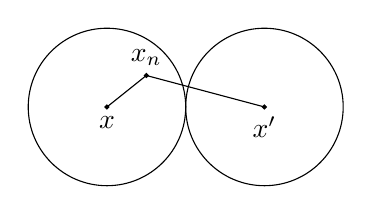
\begin{tikzpicture} 
                \draw (-1,0) circle[radius=1];
                \draw (1,0) circle[radius=1]; 
                \draw[fill] (-1,0) circle[radius=0.025] node[below]{$x$}; 
                \draw[fill] (1,0) circle[radius=0.025] node[below]{$x'$};
                \draw[fill] (-0.5,0.4) circle[radius=0.025] node[above]{$x_n$};
                \draw (-1,0) -- (-0.5,0.4); 
                \draw (-0.5,0.4) -- (1,0);
            \end{tikzpicture} 
            $f_n(x) \neq f_n (x')$ \\ 
            Mamy sprawdzić, że $F^{-1} : F[X] \to X$ jest ciągła. \\
            Jeżeli $F(y_j) \to F(y)$, to $y_j \to y$.
            Niech ciąg $(y_j)$ nie jest zbieżny do $y$. Istnieje $\varepsilon > 0 
            y_i \notin B_\varepsilon (y)$ dla nieskończenie wielu $j$. \\ 
            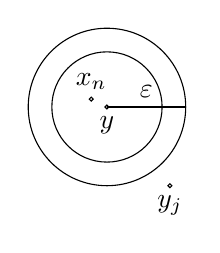
\begin{tikzpicture} 
                \draw circle[radius=1];
                \draw (0,0)--(1,0) node[midway,above]{$\varepsilon$}; 
                \draw circle[radius=0.025] node[below]{$y$};
                \draw (0.8,-1) circle[radius=0.025] node[below]{$y_j$};
                \draw circle[radius=0.7];
                \draw (-0.2,0.1) circle[radius=0.025] node[above]{$x_n$};
            \end{tikzpicture} \\ 
            Stad $F(y_j)$ nie zbiega do $F(y)$. Niech $x_n \in B_{\frac{\varepsilon}{3}} (y)$ \\
            $f_n (y) = \rho(y,x_n) < \frac{\varepsilon}{3}$ \\ 
            $f_n (y_j) = \rho(y_j,x_n) \ge \frac{2\varepsilon}{3}$ \\ 
            stąd $F(y_j)$ nie zbiega do $F(y)$ \lightning.
    \end{itemize} 
\end{dd} 

\begin{tw} Kostka Hilberta jest zwarta w metryce m. \end{tw} 
\begin{lem} 
    Jeżeli $\mathbb{N} \supseteq A_1 \supseteq \ldots \supseteq A_j \supseteq \ldots $ są nieskończone to 
    istnieje nieskończony $A \subseteq N$ taki, że $A \overset{\ast}{\subseteq} A_j$, czyli
    $A \setminus A_j$ jest skończony.
    \begin{dd} 
        Definujemy $n_1 < n_2 < \ldots < n_k < \ldots$ \\ 
        $n_k$ - pierwsza liczba ze zbioru $A_k$, która jest większa od $n_{k-1}$.
        $A = \{n_1,n_2,\ldots\}$ \hfill \qed
    \end{dd} 
\end{lem} 
\begin{dd} 
    Niech $x_n \in [0,1]^\mathbb{N}$. \\ 
    Pokażemy, że $(x_n)$ ma podciąg zbieżny. Istnieje nieskończony $A_1 \subseteq \mathbb{N}$ taki,  
    że $(x_n(1))_{n \in A_1}$ jest zbieżny do $x(1)$. Rozważmy $(x_n)_{n \in A_1}$. Istnieje 
    nieskończony $A_2 \subseteq A_1$, taki, że $(x_n (2))_{n \in A_2}$ jest zbieżny do $x(2)$. \\ 
    Definiujemy nieskończone zbiory $A_1 \supseteq A_2 \subseteq \ldots$ takie, że dla każdego 
    $j \ (x_n(j))_{n \in A_j}$ jest zbieżny do $x(j)$.
    Niech $A \overset{\ast}{\subseteq} A_j$ dla każdego $j$. Wtedy $(x_n)_{n \in A}$ jest zbieżny do 
    $x = (x(1),x(2),\ldots) \in [0,1]^\mathbb{N}$.
\end{dd} 

\begin{wn} \hfill 
    \begin{enumerate}[(1)]
        \item Każda przestrzeń metryczna ośrodkowa zanurza się w przestrzeni metrycznej zwartej
        \item Przestrzeń $X$ jest zwarta wtedy i tylko wtedy, gdy $X$ jest homeomorifczna z domkniętym
            podzbiorem $[0,1]^\mathbb{N}$.
        \item Ka każdej przestrzeni metrycznej ośrodkowej istnieje równoważna metryka całkowicie ograniczona.
    \end{enumerate}
\end{wn} 

\begin{dd} 
    \begin{enumerate}[(1)] 
        \item chyba oczywiste xD
        \item Jeżeli $X$ jest zwarta (i metryczna) to $X$ jest ośrodkowa, więc $X \hookrightarrow [0,1]^\mathbb{N}$. \\ 
            Istnieje $F: X \underset{'1-1'}{\xrightarrow{\text{ciągły}}} [0,1]^\mathbb{N}$. Wtedy 
            $F[X]$ jest zwarty, więc jest domknięty.
        \item Istnieje zanurzenie $F: X \to [0,1]^\mathbb{N}$. Metryka $m$ jest całkowicie ograniczona. \\ 
            Wtedy $\rho' (x,y) = m(F(x),F(y))$, definicjia równoważna metryce całkowicie ograniczonej.
    \end{enumerate} 
\end{dd} 
\begin{tw}[tw. Aleksandrowa]
    Dla danej przestrzeni metrycznej ośrodkowej $(X,\rho)$ NWSR: 
    \begin{enumerate}[(1)]
        \item Istnieje równoważna metryka zupełna
        \item $X$ jest homeomorficzna z pozdbiorem $[0,1]^\mathbb{N}$ typu $G_\delta$.
    \end{enumerate} 
\end{tw}
\begin{wn} Na $\mathbb{R} \setminus \mathbb{Q}$ istnieje metryka równoważna zupełna. \end{wn} 
\begin{prz} 
    $X = (0,1)$ nie jest zupełna w metryce euklidesowej, ale $\rho (x,y) = | \operatorname{arctg} x - \operatorname{arctg} y|$ jest 
    równoważna metryce zupełnej.
\end{prz} 
\begin{prz} 
    $X = \mathbb{Q}$ nie jest zuepłna w metryce euklidesowej. Dowolna metryka równoważna na $\mathbb{Q}$ nie jest zupełna. 
    $\mathbb{Q} = \bigcup\limits_{q \in \mathbb{Q}} (q)$
\end{prz}
